% GravExplainSuppMatt

\documentclass[aps,pra,superscriptaddress,reprint]{revtex4-1}
\usepackage[utf8]{inputenc}
\usepackage{amsmath,amssymb,amsthm}
\usepackage{amsfonts}
\usepackage{graphicx}
\usepackage{float}
\usepackage{mathtools}
\usepackage[usenames,dvipsnames]{xcolor}
\usepackage{hyperref}
\usepackage{textcomp}
\usepackage{subfiles}
\usepackage{comment}
\usepackage{algpseudocode}
\usepackage{lmodern}

\usepackage{silence}
\WarningFilter{revtex4-1}{Repair the float}


\newcommand{\jam}{\textcolor{magenta}}
\newcommand{\han}{\textcolor{orange}}


\begin{document}



\title{Supplementary Material for \\Continuous gravitational waves in the lab: recovering audio signals with a table-top optical microphone} 

\author{\textbf{[Authors removed for double-anonymous review.]}}

\begin{comment}

\author{James W. Gardner}
\email{u6069809@anu.edu.au}
% \affiliation{%
% College of Science, Australian National University, Acton, ACT, 2601, Australia 
% }%
\affiliation{%
ANU Centre for Gravitational Astrophysics, The Australian National University, Acton, ACT, 2601, Australia
}
\affiliation{%
OzGrav-ANU, Australian Research Council Centre of Excellence for Gravitational Wave Discovery, The Australian National University, Acton, ACT, 2601, Australia
} 
\affiliation{%
School of Physics, University of Melbourne, Parkville, Victoria, 3010, Australia
}


\author{Hannah Middleton}
\email{hannah.middleton@unimelb.edu.au}
\affiliation{%
School of Physics, University of Melbourne, Parkville, Victoria, 3010, Australia
}
\affiliation{%
Centre for Astrophysics and Supercomputing, Swinburne University of Technology, Hawthorn, Victoria 3122, Australia 
}
\affiliation{%
OzGrav-Melbourne, Australian Research Council Centre of Excellence for Gravitational Wave Discovery, Parkville, Victoria 3010, Australia
}

\author{Changrong Liu}
\affiliation{%
Department of Electrical and Electronic Engineering, University of Melbourne, Parkville, Victoria 3010, Australia
}
\affiliation{%
OzGrav-Melbourne, Australian Research Council Centre of Excellence for Gravitational Wave Discovery, Parkville, Victoria 3010, Australia
}

\author{Andrew Melatos}
\email{amelatos@unimelb.edu.au}
\affiliation{%
School of Physics, University of Melbourne, Parkville, Victoria, 3010, Australia
}
\affiliation{%
OzGrav-Melbourne, Australian Research Council Centre of Excellence for Gravitational Wave Discovery, Parkville, Victoria 3010, Australia
}


\author{Robin Evans}
\affiliation{%
Department of Electrical and Electronic Engineering, University of Melbourne, Parkville, Victoria 3010, Australia
}
\affiliation{%
OzGrav-Melbourne, Australian Research Council Centre of Excellence for Gravitational Wave Discovery, Parkville, Victoria 3010, Australia
}

\author{William Moran}
\affiliation{%
Department of Electrical and Electronic Engineering, University of Melbourne, Parkville, Victoria 3010, Australia
}


\author{Deeksha Beniwal}
\affiliation{%
Department of Physics, The University of Adelaide, South Australia, 5005, Australia
}
\affiliation{%
The Institute of Photonics and Advanced Sensing (IPAS), The University of Adelaide, South Australia, 5005, Australia
}
\affiliation{%
OzGrav-Adelaide, Australian Research Council Centre of Excellence for Gravitational Wave Discovery, South Australia, 5005, Australia
}


\author{Huy Tuong Cao}
\affiliation{%
Department of Physics, The University of Adelaide, South Australia, 5005, Australia
}
\affiliation{%
The Institute of Photonics and Advanced Sensing (IPAS), The University of Adelaide, South Australia, 5005, Australia
}
\affiliation{%
OzGrav-Adelaide, Australian Research Council Centre of Excellence for Gravitational Wave Discovery, South Australia, 5005, Australia
}

\author{Craig Ingram}
\affiliation{%
Department of Physics, The University of Adelaide, South Australia, 5005, Australia
}
\affiliation{%
The Institute of Photonics and Advanced Sensing (IPAS), The University of Adelaide, South Australia, 5005, Australia
}
\affiliation{%
OzGrav-Adelaide, Australian Research Council Centre of Excellence for Gravitational Wave Discovery, South Australia, 5005, Australia
}

\author{Daniel Brown}
\affiliation{%
Department of Physics, The University of Adelaide, South Australia, 5005, Australia
}
\affiliation{%
The Institute of Photonics and Advanced Sensing (IPAS), The University of Adelaide, South Australia, 5005, Australia
}
\affiliation{%
OzGrav-Adelaide, Australian Research Council Centre of Excellence for Gravitational Wave Discovery, South Australia, 5005, Australia
}

\author{Sebastian Ng}
\affiliation{%
Department of Physics, The University of Adelaide, South Australia, 5005, Australia
}
\affiliation{%
The Institute of Photonics and Advanced Sensing (IPAS), The University of Adelaide, South Australia, 5005, Australia
}
\affiliation{%
OzGrav-Adelaide, Australian Research Council Centre of Excellence for Gravitational Wave Discovery, South Australia, 5005, Australia
}
\end{comment}








\maketitle

\section{Optical microphone signal processing}


In Section~V in the main article, we use the interferometer as an optical microphone; audio signals are used to vibrate the interferometer mirrors, the changing interference pattern is recorded, and we aim to recover the original signal from the resulting timeseries data.
In this Supplementary Material, we include a selection of signal processing techniques applied to the data which may be considered for undergraduate laboratory examples. 
We start with some na{\"i}ve approaches and then move to traditional signal processing filters (band-passing and cascaded notches). 
We finish by combining these with advanced statistical techniques (Wiener filter and the logMMSE estimator). 
As an example, we test all of these filters on the same $1\,{\rm s}$ long speech recording.
For more information about the techniques used here see Refs.~\cite{Mitra:2011, Lyons:2011, Stein:2000, OpenheimSchaferBuck:1999, PrakisManolakis:1996,10.5555/151045}.

\begin{figure*}
	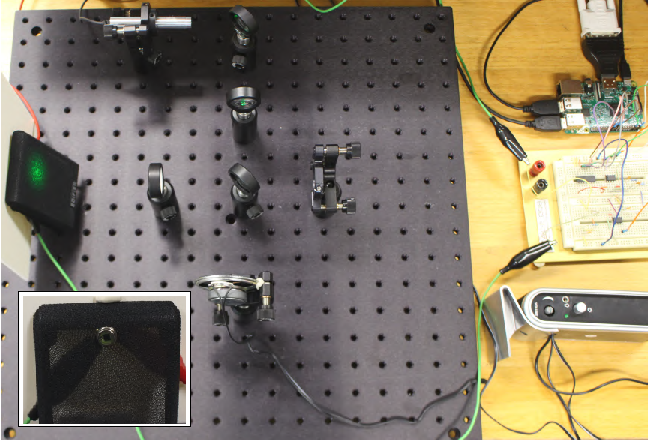
\includegraphics[height=0.41\textwidth]{figures/setup_pic2.pdf}
	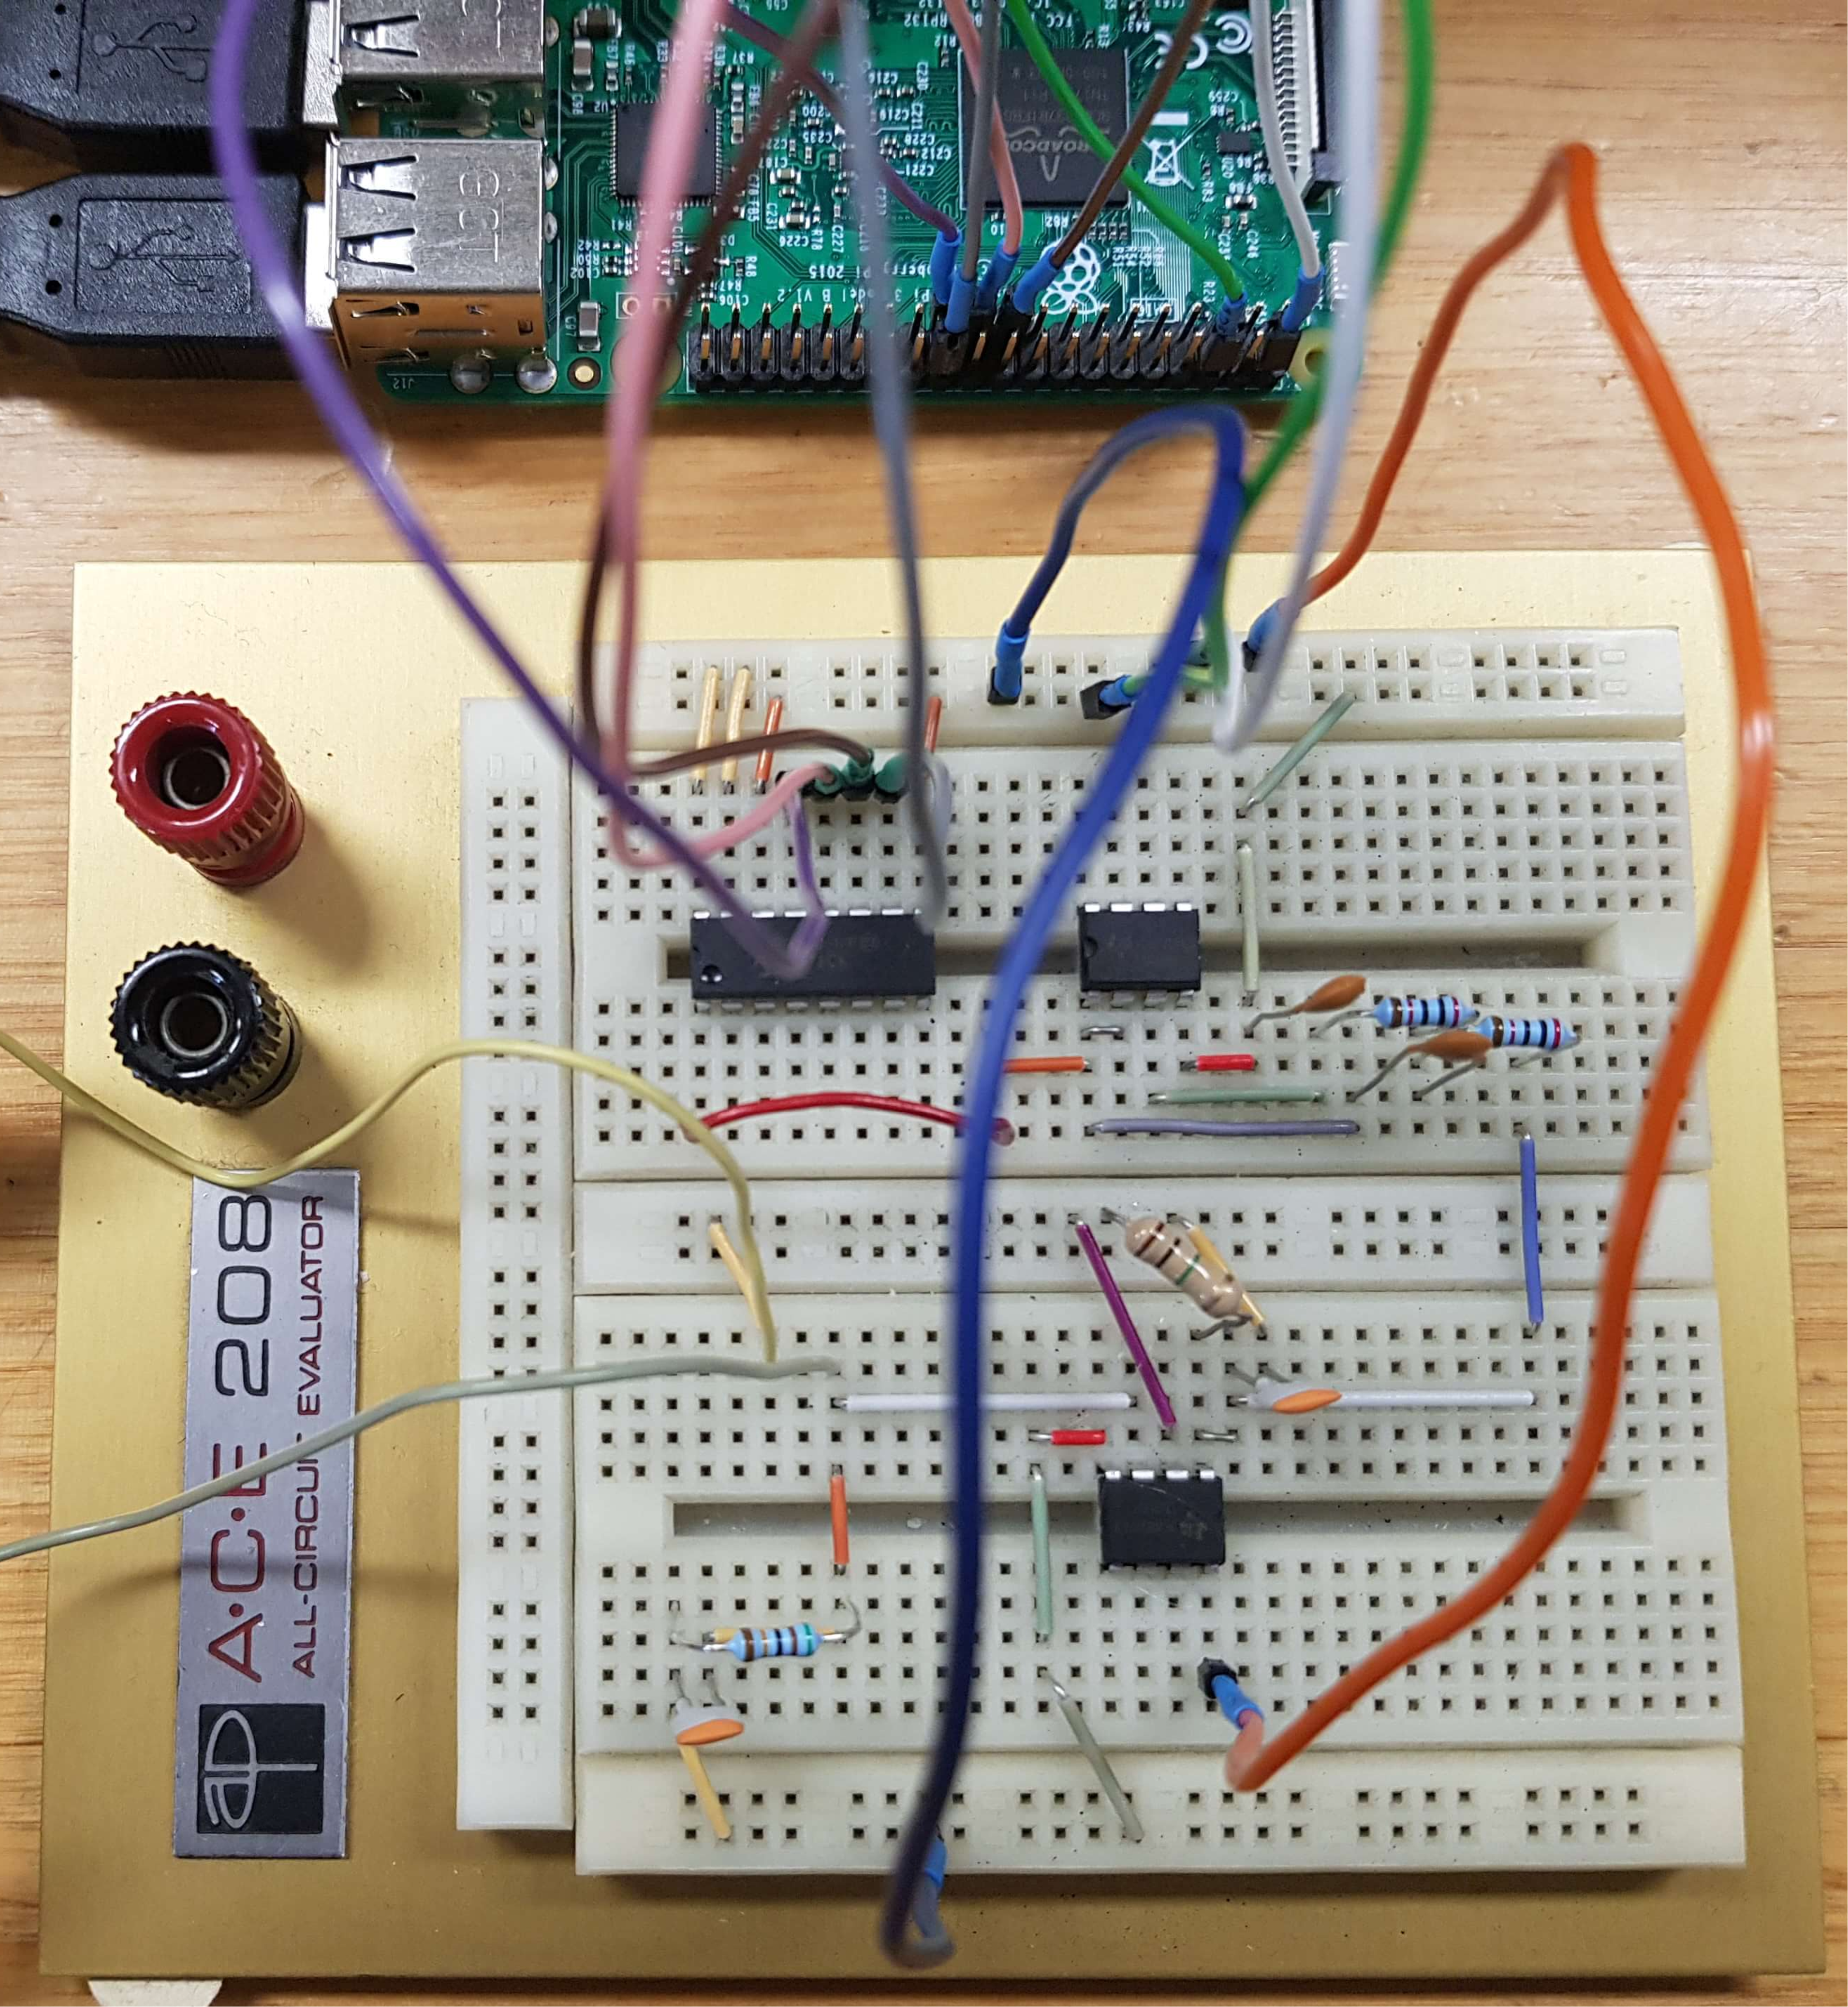
\includegraphics[height=0.41\textwidth]{figures/circuit_pic3.pdf}
	\caption{
Left: A photograph of the optical microphone with an inset of the photodiode. The Michelson interferometer is shown on the left and the circuit and Raspberry Pi on the right. In the main image, the photodiode is placed behind a cloth screen as explained in the main article. The inset shows a face-on view of the photodiode with the cloth screen removed. 
Right: A photograph of the photodiode circuit assembled on a breadboard. The leads from the photodiode enter from the left of the picture. The Raspberry Pi is shown at the top of the picture.
}
	\label{fig:photographs_of_optical_microphone_and_circuit}
\end{figure*}


All analysis is done using the photodiode set-up as described in Section~V.A. in the main article. 
A photograph of the equipment is shown in Fig.~\ref{fig:photographs_of_optical_microphone_and_circuit} with the interferometer and circuit shown on the left and right, respectively. 


\begin{figure}
	\begin{center}
    %% trim order is <left> <lower> <right> <upper>
    % height=0.5\textheight,trim={1cm 4.5cm 0.4cm 3.5cm},clip
	\includegraphics[width=.5\textwidth]
% trim={1cm 3cm 1cm 1cm}]
{figures/combined_results_full_melatos_labelled.pdf}
%notch_and_wiener_superplot_v2.pdf}
	\end{center}
	\caption{\label{fig:op_mic_results}
	%\jam{Fig.2 should be combined with Fig.6 using combined\_results\_full\_melatos\_labelled.pdf}
	Timeseries (left column) and frequency spectrum (right column) results for the background subtraction, notch, and Wiener filters.
    The top two rows are the input signal and raw output (identical to the top two rows in Fig.~7 in the main article).  
    The third row shows a background noise recording from the optical microphone when no audio signal is played. 
    The fourth row shows the result of subtracting the background noise spectrum in the third row from the recording in the second row. 
	The fifth and sixth rows show the results of applying the cascaded-notch filter and Wiener filter respectively.
    The seventh shows the results of applying both the cascaded-notch and Wiener filter (identical to the third row in Fig.~7 in the main article).
    The eighth row shows the results of applying the logMMSE estimator (identical to the fourth row in Fig.~7 in the main article). 
	}
\end{figure}



Results for a selection of filters are collated in Fig.~\ref{fig:op_mic_results}, which we refer to throughout this Supplementary Material. 
The left and right columns show timeseries and Fourier spectrum results, respectively. 
The first and second rows in Fig.~\ref{fig:op_mic_results} show the original source signal and the raw optical microphone recording, respectively. 
The following sections describe a sequence of analysis techniques and a selection of their results is presented in Fig.~\ref{fig:op_mic_results}.



\subsection{Background noise subtraction}

The first technique we consider is quite intuitive: we try to remove noise by directly subtracting the background noise from the recorded spectrum. 
The third row in Fig.~\ref{fig:op_mic_results} shows the interferometer background noise when there is no input signal.
The fourth row shows the spectrum obtained after subtracting the background noise spectrum, i.e.\ the result of subtracting the third row from the second row. 
We see no obvious improvement, which may be attributed to a time-variant noise spectrum, the cause of which is unidentified. 



\subsection{Rectangular comb filter}

Since the mains harmonics are present in the signal, we try to selectively remove them.
However, simply zeroing the frequency bins corresponding to the harmonics of the $50\,{\rm Hz}$ mains signal is unsuccessful. 
This effectively multiplies the spectrum by a rectangular comb filter. 
It does remove the mains harmonics, but audibly ruins the rest of the signal due to lack of smoothness. 
This is because applying a filter in frequency space is equivalent to convolving the time-domain signal with the inverse Fourier transform of that filter. 
The inverse Fourier transform of a rectangular comb filter (a set of boxcars) is some combination of sinc functions, which significantly corrupt the signal. 
See also Section~\ref{sec:notch} where we explore a notch filter. 



\subsection{High-pass filter}

A high-pass filter smoothly attenuates frequencies below some cut-off frequency. 
Applying a high-pass filter, with a cut-off frequency around $150\,{\rm Hz}$, to the signal spectrum works well at removing the $50\,{\rm Hz}$ and $100\,{\rm Hz}$ harmonics. However, the mains harmonics above $100\,{\rm Hz}$ remain. A high-pass filter with a higher cut-off can be used to mitigate this issue. However, it makes the played-back signal unrecognizable as the region above $100\,{\rm Hz}$ carries a lot of the fundamental frequencies of speech and music~\cite{speech_intelligibility}.
Often in speech processing, the logarithm of the signal is taken since the amplitude information seems to be more important to intelligibility than the phase information to the human ear~\cite{SubjectiveComparison}. However, applying a high-pass filter to the logarithm of the signal spectrum does not significantly improve on the above simple high-pass filter.


\subsection{Butterworth band-pass filter}

\begin{figure}
	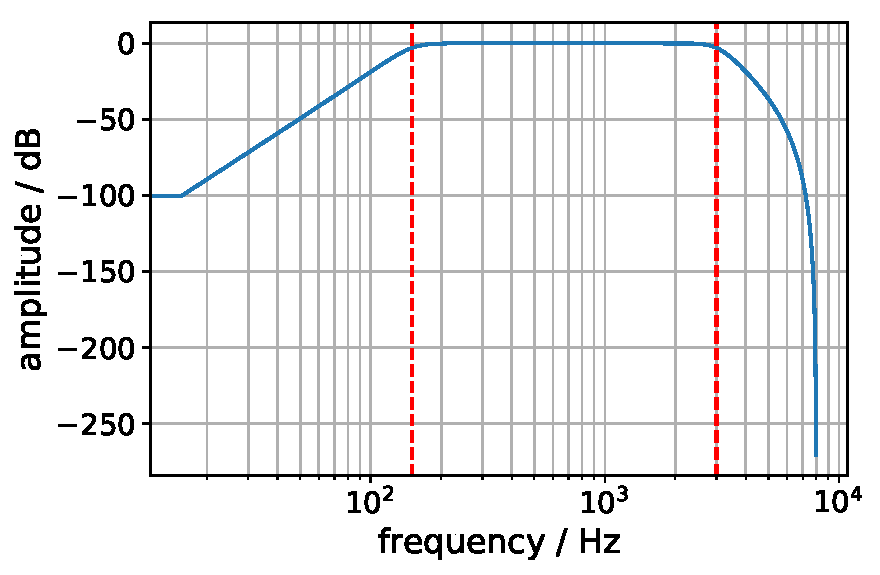
\includegraphics[width=0.5\textwidth]{figures/butterworth_150_3000.pdf}
	\caption{
Butterworth bandpass filter frequency response. 
%Any amplitude below $-3\,{\rm dB}$ is significant attenuation (less than half the power at that frequency remains). 
% suggest removing as -3db is hard to judge on the figure and I think the attenuation outside the frequency range is the key point to get across here
The red, dashed vertical lines show the band limits of $150\,{\rm Hz}$ and $3\,{\rm kHz}$. Note the flat response within the band characteristic of the Butterworth filter.}
	\label{fig:butterworth}
\end{figure}

A general band-pass filter combines a high-pass filter and a low-pass filter to smoothly attenuate frequencies outside of some band (alt.\ pass-band). A Butterworth band-pass filter is a particular band-pass filter such that the frequency response (the attenuation at each frequency) is ``maximally flat'' within the band. The Butterworth low-pass component is given by %Eqn.~\ref{eq:butterworth}

\begin{equation}
\label{eq:butterworth}
H(f) = \left[1+\varepsilon^2 \left( \frac{f}{f_c} \right)^{2n}\right]^{-1/2},
\end{equation}
and is combined with a similar high-pass filter to form the band-pass filter.
In Eqn.~\ref{eq:butterworth}, $f_c$ is the cut-off frequency of the low-pass Butterworth filter, $\varepsilon$ is the gain, and $n$ is the order of the filter which determines how quickly the response rolls off past the cut-off frequency. Fig.~\ref{fig:butterworth} shows the frequency response of the filter used here: a fifth order ($n = 5$) Butterworth filter with a pass-band of $(150\,{\rm Hz}$, $3\,{\rm kHz})$. This high frequency ($3\,{\rm kHz}$) cut-off is chosen since the frequencies important for speech generally lie below $2\,{\rm kHz}$~\cite{speech_intelligibility}.

The effect of applying this filter to the background noise PSD can be seen in the bottom panel in Fig.~\ref{fig:psd_noise}. The Butterworth band-pass filter reduces the amplitude of mains harmonics below $150\,{\rm Hz}$ and suppresses unrelated noise sources above $3\,{\rm kHz}$. However, it does not address the issue of mains harmonics above $150\,{\rm Hz}$ (i.e.\ those in the pass-band). In the following section, we experiment with a cascade notch filter to address this.

\begin{figure}
	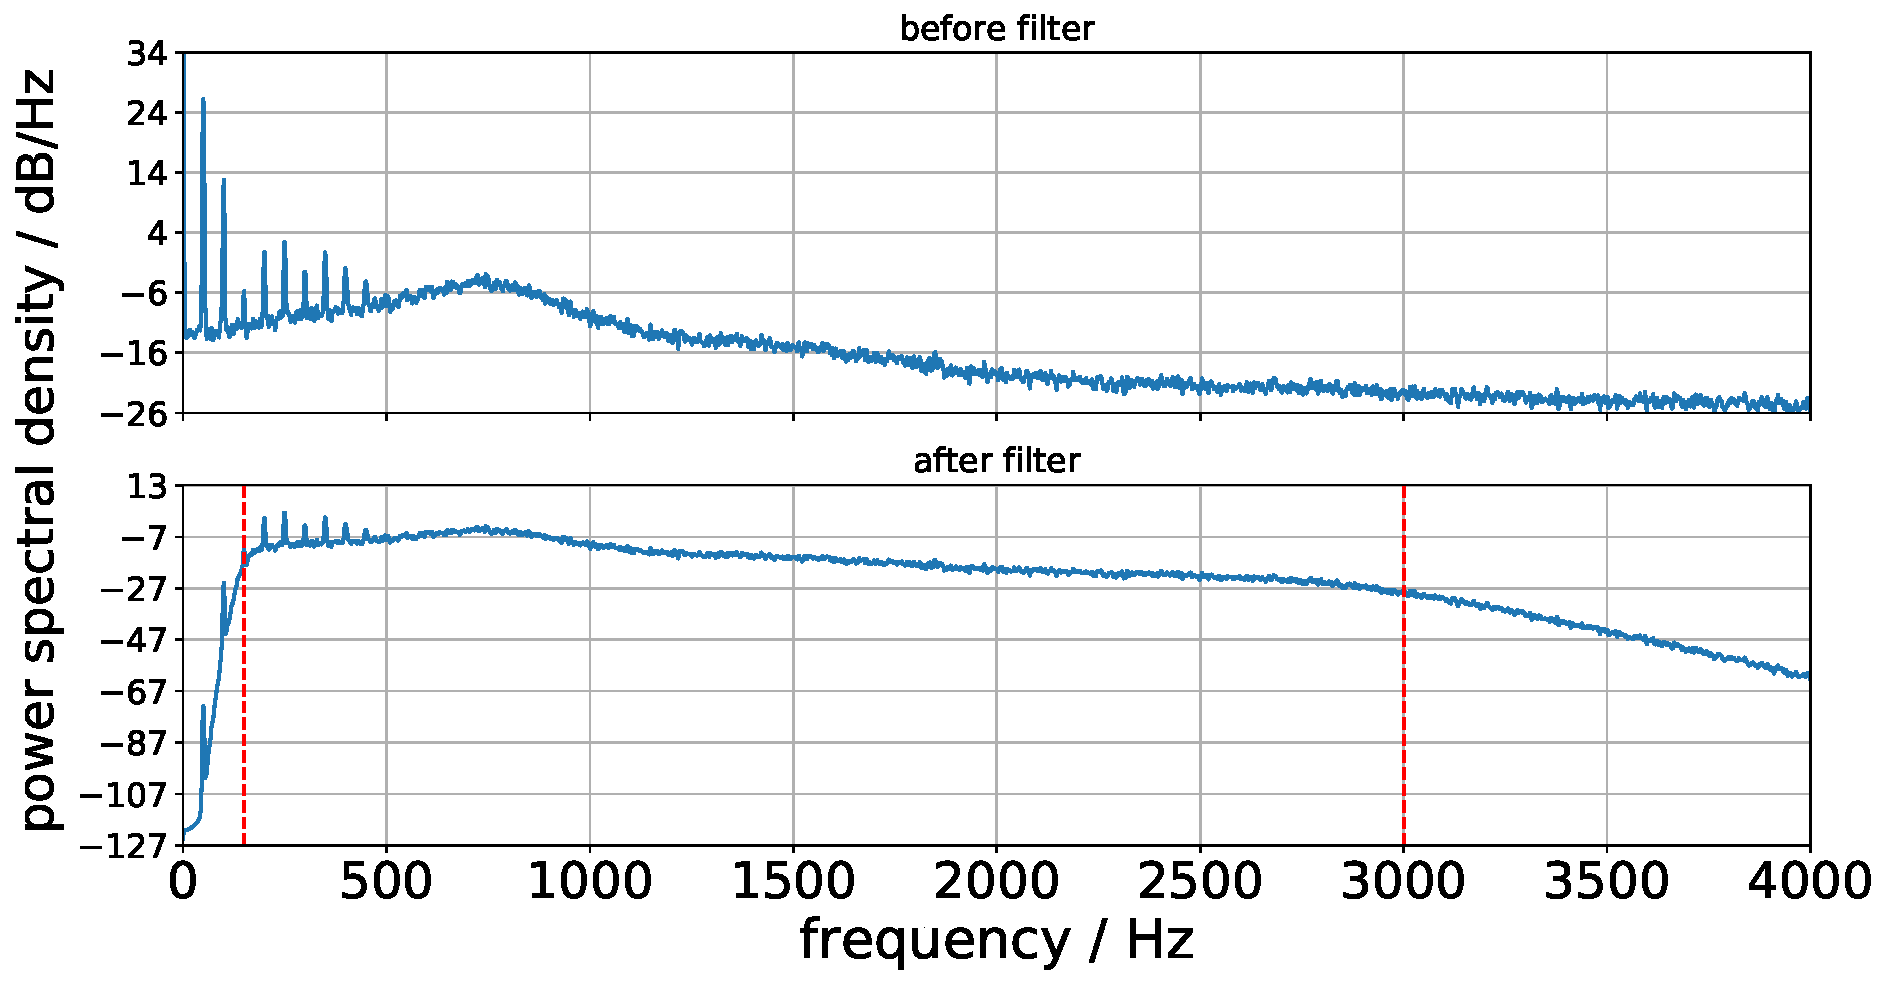
\includegraphics[width=.5\textwidth]{figures/psd_butterworth_14_6.pdf}
	\caption{\label{fig:psd_noise}
Top: power spectral density (PSD) of background noise from the optical microphone (with the speaker off). 
Bottom: the PSD after applying a Butterworth bandpass filter (bottom panel) between the two frequencies marked with red, dashed lines. 
We see strong power from the $50\,{\rm Hz}$ mains hum and its harmonics (most likely from the photodiode circuit and the room’s lighting and cooling). Otherwise, the PSD is fairly white. 
After filtering, we see significant attenuation (at least 3~dB) of all frequencies outside the band.
However, the filter has little change on the harmonics within the band.
The sharp drop-off at low frequencies, around 100~dB near 0~Hz, is due to stronger attenuation far from the band and would appear shallower if shown against a logarithmic scale for frequency as in Fig.~\ref{fig:butterworth}.
}
\end{figure}


\subsection{Cascade notch filter}

\label{sec:notch}
\begin{figure}
\begin{center}
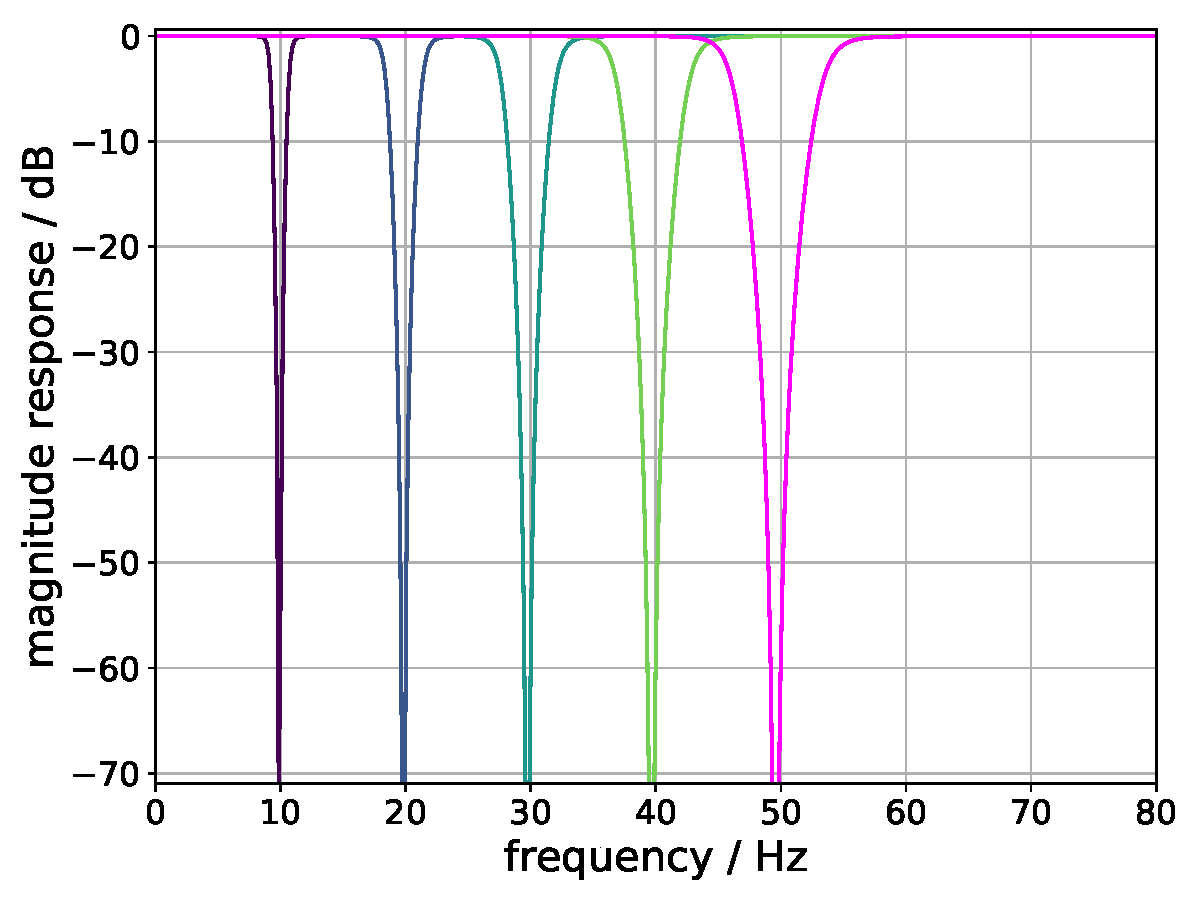
\includegraphics[width=.5\textwidth]{figures/cascaded_notch_response_plot.pdf}
\end{center}
\caption{\label{fig:notchMagResponse}
Amplitude (magnitude) response for the first five notches of fifteen for the cascaded notch filter described by Eqs.~\ref{eqn:notch} and~\ref{eqn:notch15}. 
}
\end{figure}

One method to remove mains noise and its harmonics is to use a sequence of notch filters centered at each of the frequency bins we want to remove. This sequence is known as a ``cascade'' of notches. Here, the notches are smooth in comparison to the na{\"i}ve zeroing of each frequency (which looks like a rectangular comb). 

The impulse response describes the reaction of a system to an input signal as a function of time. 
If a system is linear and time-invariant, the output signals are completely determined for any input signal using the impulse response. 
Finite impulse response (FIRs) filters have finite length (they equal zero outside of a finite range). 
In contrast, an infinite impulse response (IIR) filter has infinite length due to feedback. 
Typically FIR filters outperform IIR filters as they are always stable. 
However, IIR filters normally require fewer coefficients which in turn speeds up signal processing in comparison to FIR filters. 


In this work, we opt for an IIR notch filter. 
We write the filter in the form of a Z-transform, in which a discrete-time signal is converted to the complex frequency domain $z=e^{jf}$. 
The IIR notch filter we use here is given by~\citep{10.5555/541204}, 
\begin{equation}
    \label{eqn:notch}
    H(z)=\frac{1+\alpha}{2}\frac{1-2\beta z^{-1}+z^{-2}}{1-\beta(1+\alpha)z^{-1}+\alpha z^{-2}}\,,
\end{equation}
where $\alpha$ and $\beta$ are parameters that control the filter. 
These parameters determine $w_0=\cos^{-1}(\beta)$, the frequency that is completely attenuated (zeroed or ``notched'') at the centre of the notch, and $B_w=\cos^{-1}[2\alpha/(1+\alpha^2)]$, the bandwidth of the notch which determines how quickly the response changes around the notched frequency.
We find that a sequence of $15$ notches works well here, with the $k^\mathrm{th}$ notch centered on the $k^\mathrm{th}$ harmonic of the $50\,{\rm Hz}$ mains signal, where $k=0,2,\dots,14$. 
We choose the bandwidth and order (here order six) of each notch to avoid disturbing useful signals while still allowing for uncertainty in the location of each harmonic of the mains signal. The response of this cascaded notch filter $H(z)$ is the product of the responses of each of the individual $H_k(z)$ notches,
\begin{equation}
    \label{eqn:notch15}
    H(z) = \prod_{k=0}^{14} H_k(z).
\end{equation}

We use the built-in MATLAB filter design toolbox in this work~\cite{MATLAB}. 
The amplitude (magnitude) response of the first five notch filters is shown in Fig.~\ref{fig:notchMagResponse}. 
The time series and spectrum obtained after applying the cascade notch filter to the speech recording are shown in the fifth row in Fig.~\ref{fig:op_mic_results}.
We see that the mains harmonics are significantly attenuated compared to the background-subtracted results shown in the fourth row in Fig.~\ref{fig:op_mic_results}.

Although the notch filter removes much of the mains hum sound, the filtered recording is not intelligible. Qualitatively, it sounds more like a drum than a human voice. This is due to the loss of voice information under the filter.
To overcome this, we turn to more advanced techniques, starting with the Wiener filter. Instead of just passively filtering different frequencies, this statistical technique optimizes an estimate of the original signal. 






\subsection{Wiener filter}
\label{sec:Wiener}

A Wiener filter is an advanced statistical technique that estimates the injected signal given prior information about the injected spectrum and the reference spectrum of the background noise. 
The observed noisy speech signal sequence is given as $\mathbf{x}=(x(0),\dots, x(N-1))$, where $N$ is the length of the data sequence and $\mathbf{x}$ is the sum of the original injected signal $\mathbf{s}=(s(0),\dots,s(N-1))$, and the noise sequence $\mathbf{w}=(w(0),\dots,w(N-1))$, 
\begin{equation}
    \mathbf{x}=\mathbf{s}+\mathbf{w}\,.
\end{equation}
Given $\textbf{x}$, our goal is to make an estimate $\hat{\textbf{s}}$ of the original signal $\textbf{s}$ such that we minimise the Bayesian mean-square error (BMSE) between the two, defined as 
\begin{equation}
\label{eq:BMSE}
\text{BMSE}(\hat{\textbf{s}})=E[(\textbf{s}-\hat{\textbf{s}})^2]\,.
\end{equation}
If we assume that: i) $\textbf{x}$ is ``wide sense stationary''~\footnote{ A random process $\{x(t)\}$ is wide sense stationary if, for all $t_1,t_2 \in \mathbb{R}$, (1) its mean is time invariant, i.e., $\mu_x(t_1)=\mu_x(t_2)=\text{constant}$; and (2) the autocorrelation depends only on the time difference, i.e., $R_x(t_1,t_2)=R_x(\tau),\tau=t_1-t_2$.} with zero mean; ii) the signal $\textbf{s}$ has a mean of zero; and iii) the noise $\textbf{w}$ is uncorrelated with the signal $\textbf{s}$, we can further express $\hat{\textbf{s}}$ to be a linear combination of present and past observed data
\begin{equation}
\hat{{s}}[n]=\sum_{k=0}^{n}h[k]x[n-k]\,,
\end{equation}
where $\textbf{h}=(h(0),\dots h(n))$ represents the coefficients of an $n$th order Wiener filter.
The famous Wiener-Hopf equation~\citep{noble1959methods} allows us to determine $\textbf{h}$, as\begin{equation}
\label{eqn:wiener-hopf}
\begin{bmatrix}  
r_{xx}[0]&r_{xx}[1]&\dots& r_{xx}[n]\\
r_{xx}[1]&r_{xx}[0]&\dots &r_{xx}[n-1]\\
\vdots&\vdots&\ddots&\vdots\\
r_{xx}[n]&r_{xx}[n-1]&\dots &r_{xx}[0]
\end{bmatrix}
\begin{bmatrix}
h[0]\\
h[1]\\
\vdots\\
h[n]
\end{bmatrix}=
\begin{bmatrix}
r_{ss}[0]\\
r_{ss}[1]\\
\vdots\\
r_{ss}[n]
\end{bmatrix}\,,
\end{equation}
where $r_{xx}$ and $r_{ss}$ are the auto-correlation functions of $\mathbf{x}$ and $\mathbf{s}$ between timestep $i$ and $i+n$, 
%\begin{equation*}
%\left\{ 
\begin{eqnarray} 
r_{xx}[n] &~=~& E[x(i)~x(i+n)] \,,\\
r_{ss}[n] &~=~& E[s(i)~s(i+n)] \,.
%r_{xx}[n] &=& E[x(i)\, &x(i+n)] \\ 
%r_{ss}[n] &=& E[s(i)\, &s(i+n)] 
\end{eqnarray} 
%\right\}  
%\end{equation*}



If we let the Wiener filter be non-causal (i.e. we estimate the current signal based on both past \emph{and future} observations), then we can represent Eqn.~\ref{eqn:wiener-hopf} in the frequency domain as
\begin{equation}
\label{eqn:wiener}
    H(f)=\frac{P_{ss}(f)}{P_{xx}(f)}=\frac{P_{ss}(f)}{P_{ss}(f)+P_{ww}(f)}\,,
\end{equation}
where $P_{xx}(f), P_{ss}(f), P_{ww}(f)$ are the spectra of the observed noisy data, the injected signal, and the background noise, respectively. Intuitively, from Eqn.~\ref{eqn:wiener}, we can see that the non-causal Wiener filter amplifies the input signal where the signal to noise ratio (SNR) is high and attenuates the signal where the SNR is low. The causal Wiener filter (which only makes estimates based on past observations) is similar. A more detailed analysis of both kinds of Wiener filters can be found in Ref.~\citep{10.5555/151045}.


In this work, we construct a higher-order causal Wiener filter based on Eqn.~\ref{eqn:wiener-hopf}. A higher-order Wiener filter provides greater smoothing of the input signal but also increases the computational memory required. For this work, we choose a Wiener filter of order $n=100$ as it provides a reasonable balance between smoothing and efficiency. The timeseries and frequency spectrum after applying the Wiener filter are shown in the sixth row in Fig.~\ref{fig:op_mic_results}.
We see a significant improvement in the timeseries of the recovered signal, however, a strong noise hum persists, audibly. 


\subsection{Combined notch and Wiener filter}

Here, we experiment with applying a combination of the cascaded notch and the Wiener filter to the recorded speech signal. 
The results of this analysis also are described in Section V.C. in the main article. 


The Wiener filter makes use of statistical information from the speech data and noise. It amplifies the part of the signal with high SNR while suppressing the parts with low SNR (see above Sec.~\ref{sec:Wiener}). It is implemented in the form of a finite response filter, which ensures linear phase response and stability (both desirable), but at the cost of high orders computationally. By comparison, the notch filter is based on directly removing the unwanted frequency components. It is implemented in the form of an infinite impulse response filter. Although it significantly decreases the order of the overall filter, it unavoidably introduces nonlinear phase and instability. 


By combining the notch and Wiener filter, we can trade-off between the two and achieve an overall better performance, as can be seen in the seventh row in Fig.~\ref{fig:op_mic_results}.
The filtered voice after the combined notch and Wiener filter is enhanced compared to either alone. 
The mains noise is all but removed and more voice information is retained. 
However, the recovered voice still sounds muffled and is not understandable.





\subsection{logMMSE estimator}
\label{sec:logmmse}

\begin{comment}
\begin{figure*}
	%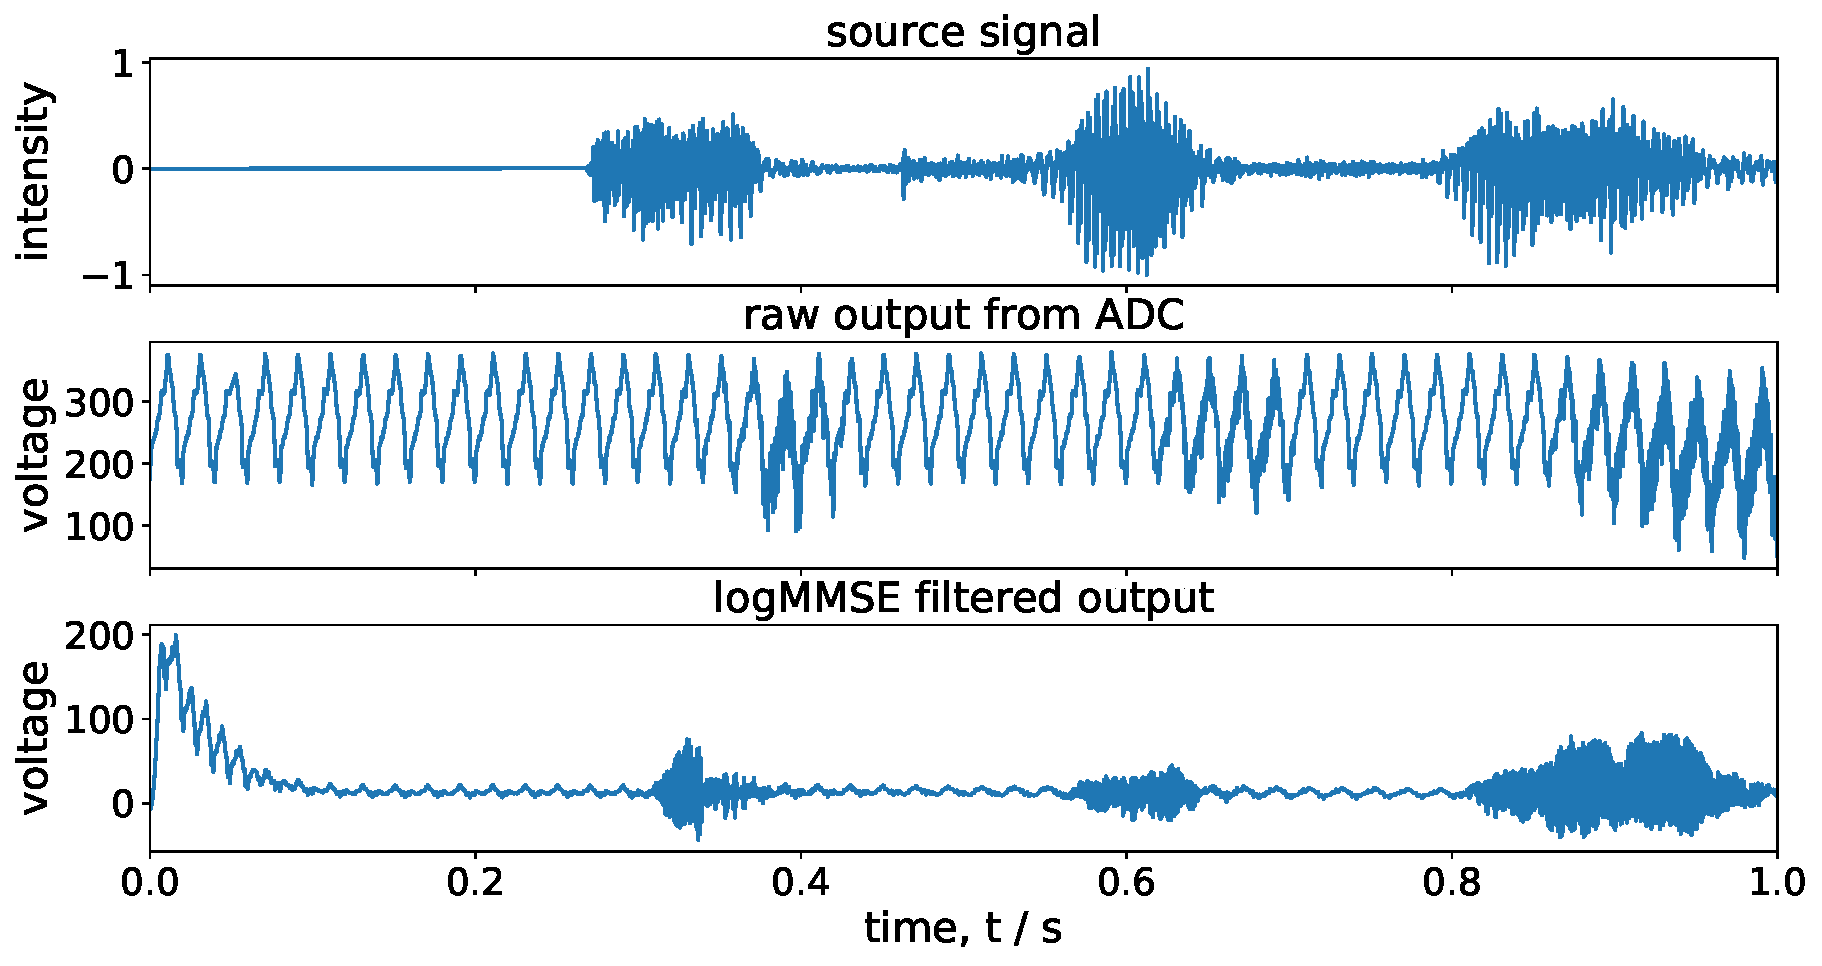
\includegraphics[width=0.49\textwidth]{figures/combined_timeseries_melatos_shift_source.pdf}
	%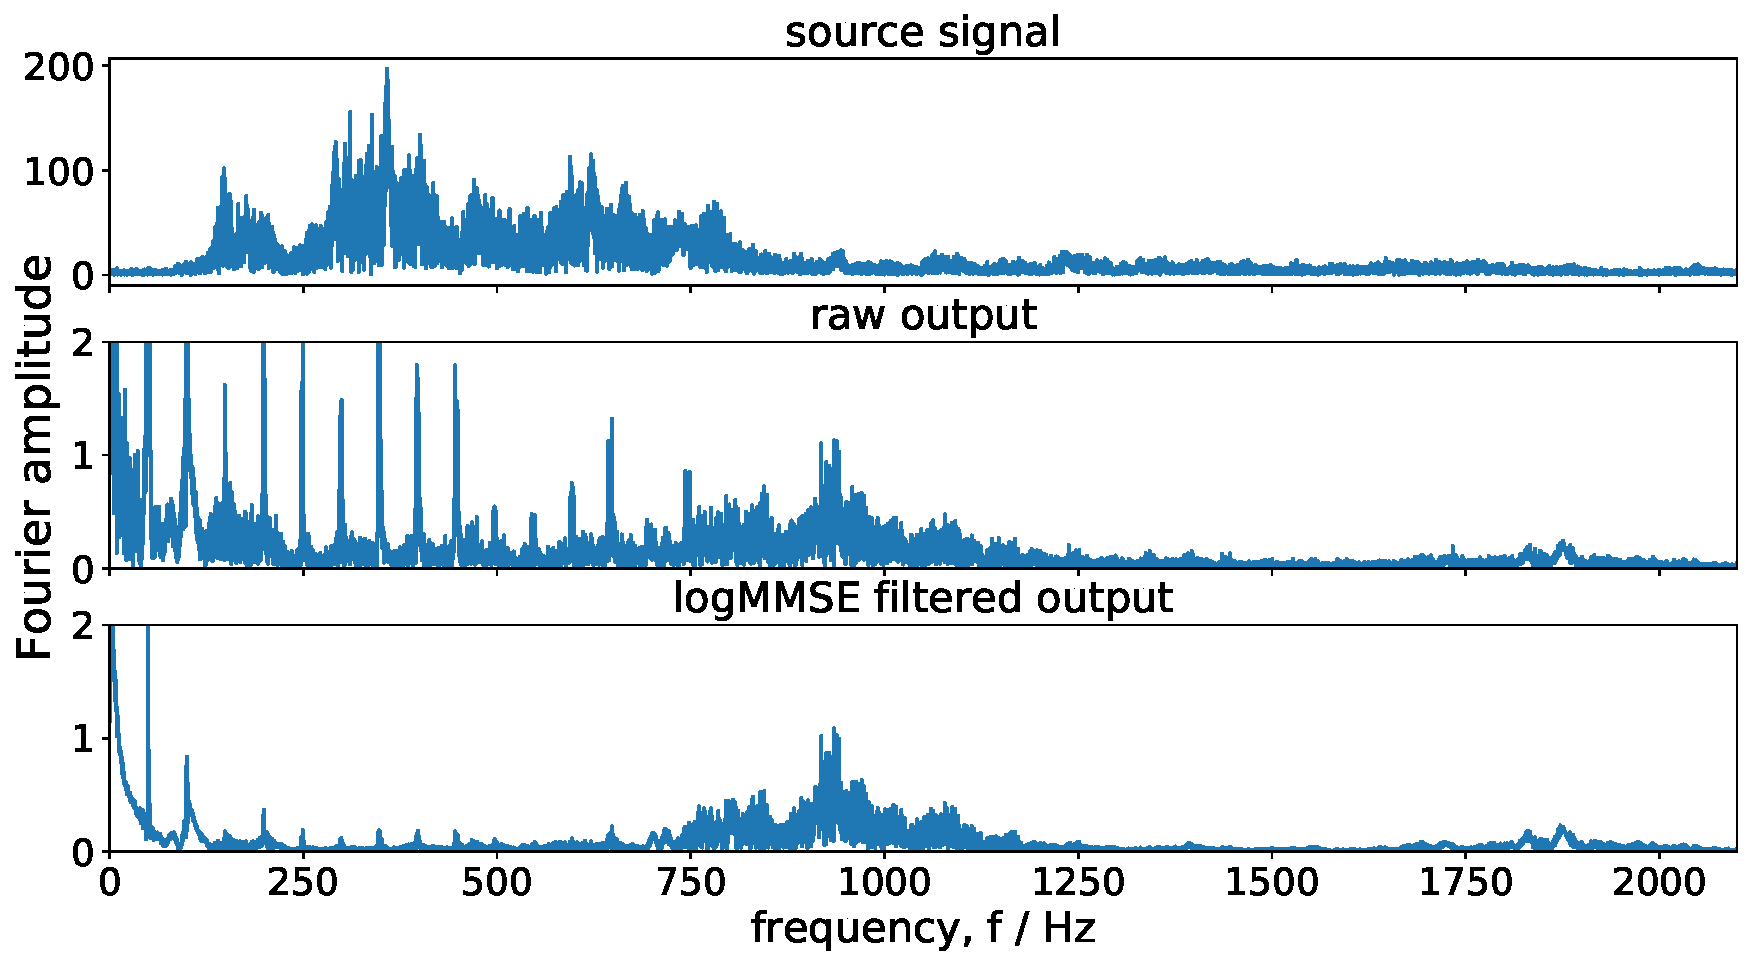
\includegraphics[width=0.49\textwidth]{figures/combined_spectrum_melatos.pdf}
    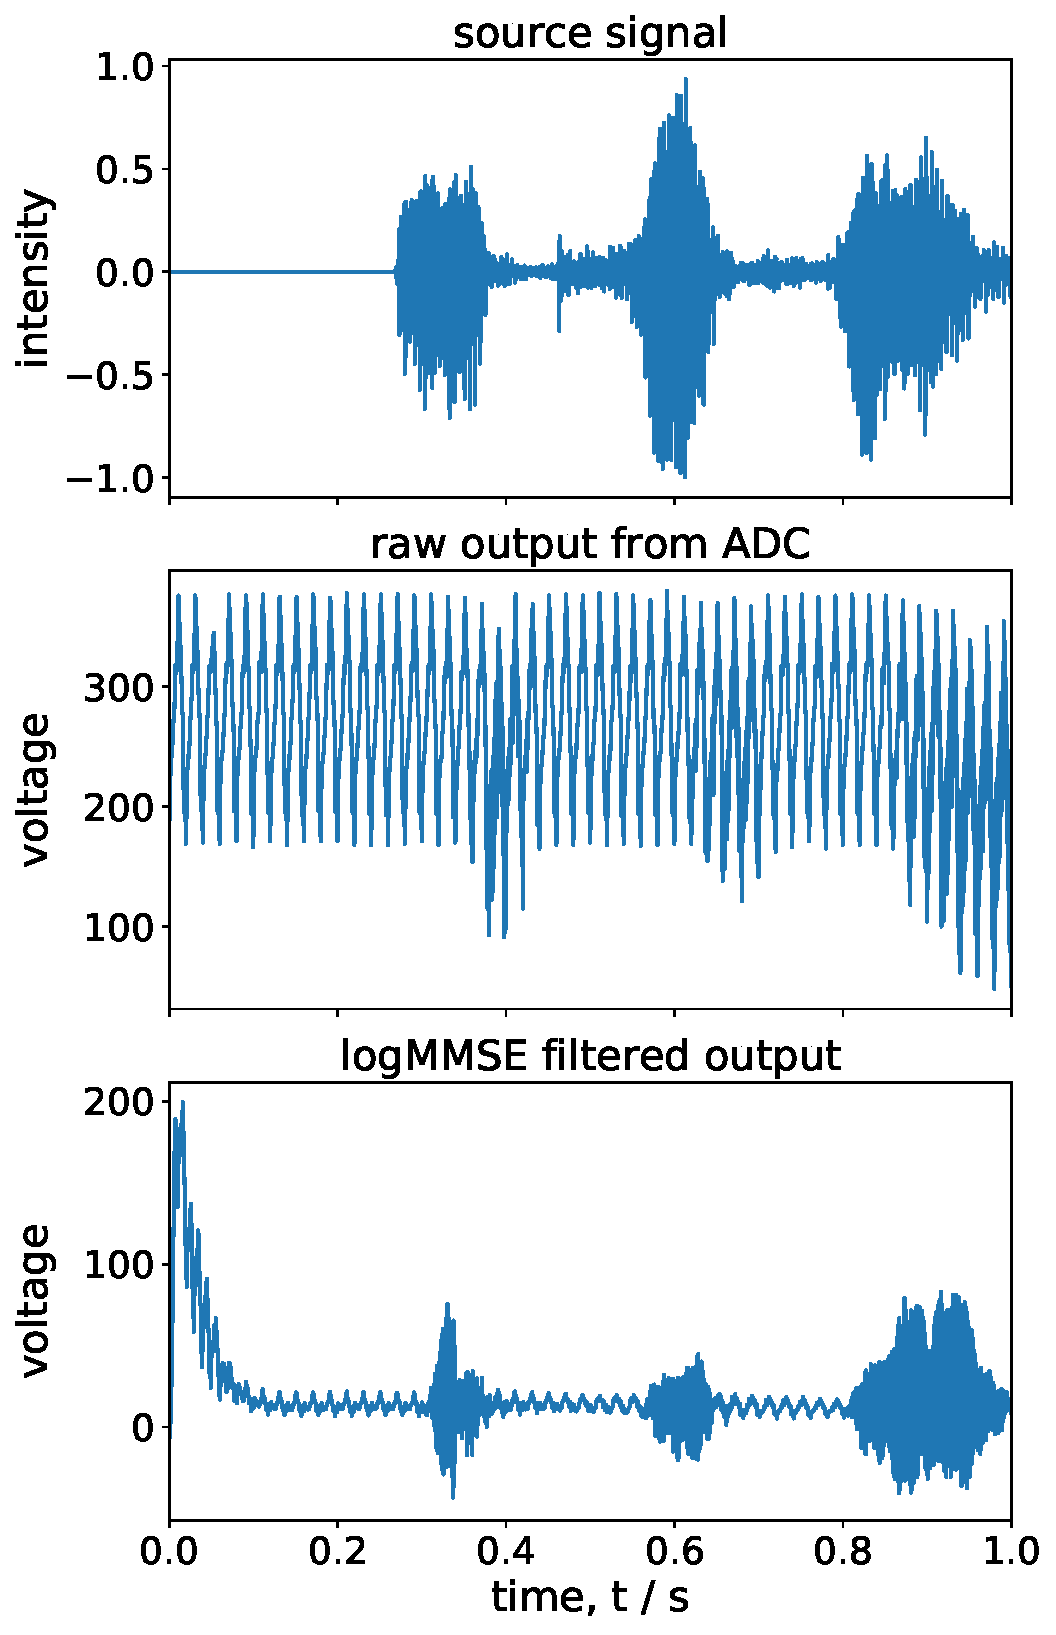
\includegraphics[height=0.57\textheight]{figures/combined_timeseries_melatos_shift_source_tall.pdf}
    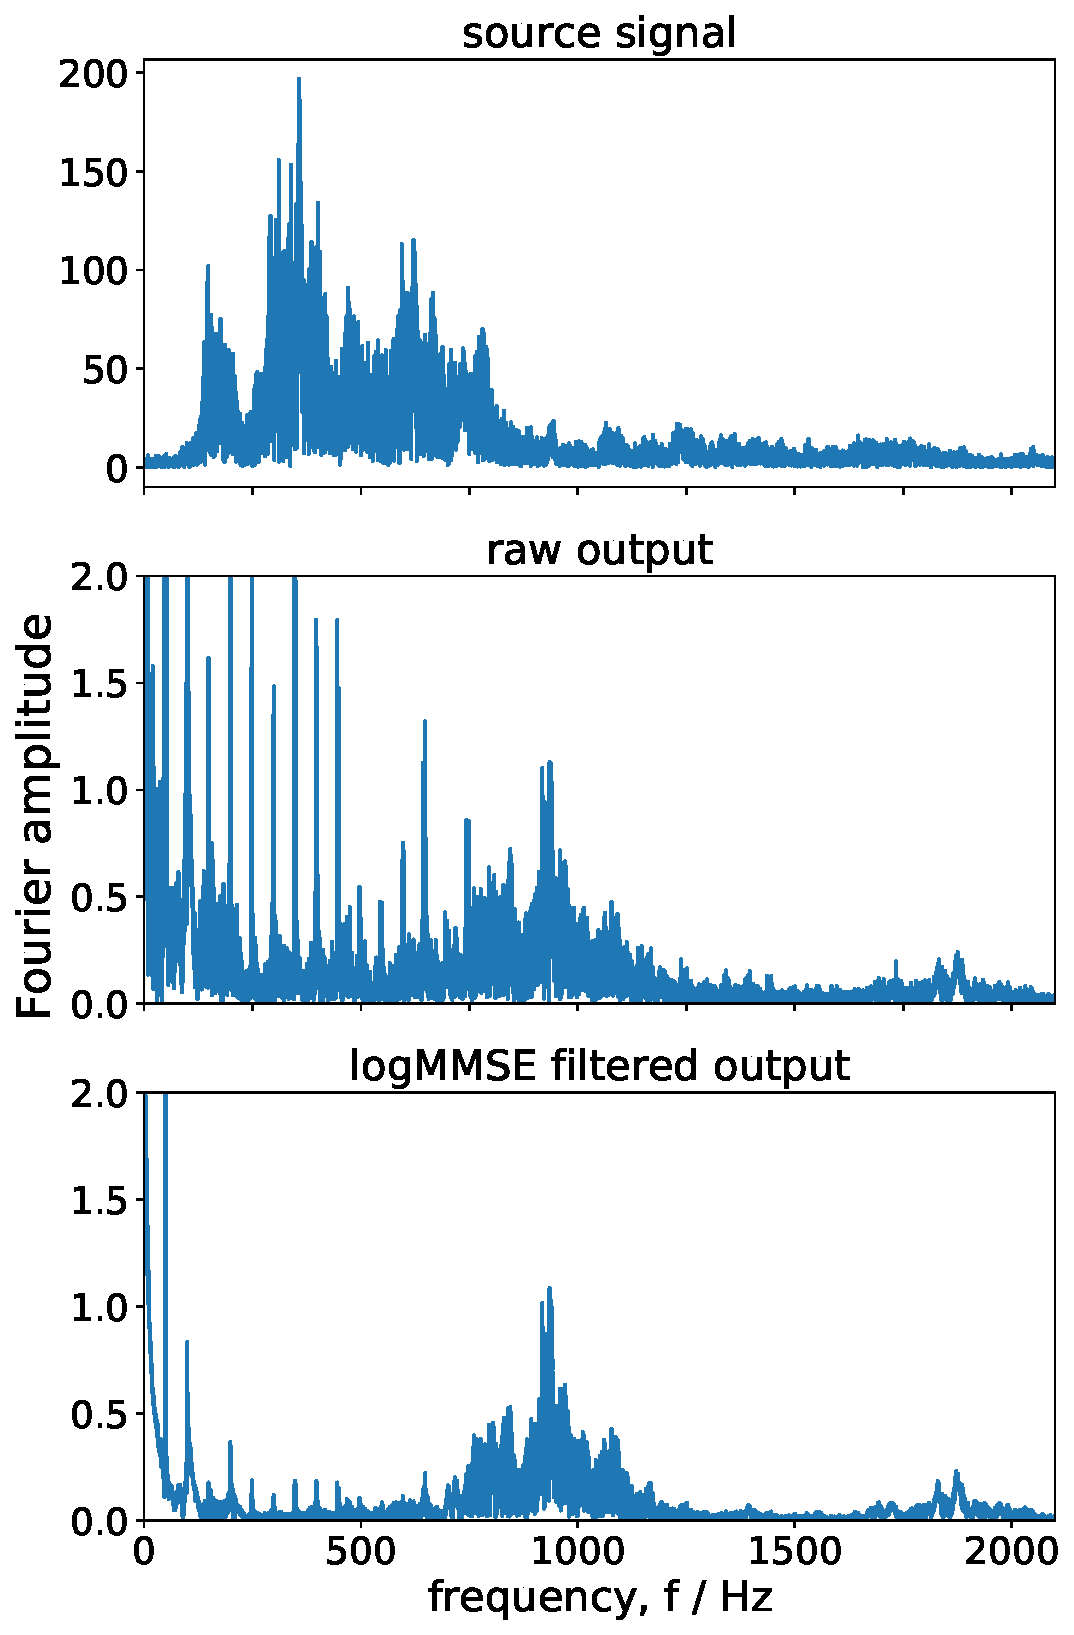
\includegraphics[height=0.57\textheight]{figures/combined_spectrum_melatos_tall.pdf}
    \caption{\label{fig:logMMSE_timeseries_freqspectrum}
\jam{Fig.2 should be combined with Fig.6 using combined\_results\_full\_melatos\_labelled.pdf}    - done 
Timeseries (left column) and frequency spectrum (right columns) results with the logMMSE estimator. 
The original source signal and optical microphone recording in the top and middle panels respectively are for comparison and are identical to those shown in the top two panels in Fig.~\ref{fig:BackgroundNotchWienerCombined} (again, the source signal is shifted by $0.12\,{\rm s}$). 
The bottom-left panel shows the timeseries of the recording after filtering with the logMMSE estimator, where the rise at the start of the timeseries is expected when filtering a signal of finite duration.
The bottom-right panel shows the corresponding frequency spectrum with the logMMSE estimator. 
The spectrum shows only a detail of the total frequency domain (there is little activity at higher frequencies) and has truncated peaks at amplitude $2$ which otherwise dominate the plot. 
The change in scale from the top panel is not of concern as the ear hears the relative frequency content and normalisation of the timeseries fixes any scaling. 
    }
\end{figure*}
\end{comment}



Speech enhancement of noisy channels is a classic problem in signal processing. 
In Ref.~\cite{SubjectiveComparison}, a comparison is made of $13$ speech enhancement methods, finding the log minimum mean-square error (logMMSE) estimator to be the best, qualitatively, at recovering speech. 
This estimator is based on speech enhancement techniques discussed in Ref.~\cite{Ephraim1984SpeechEU_logMMSE} and minimizes the mean-square error (MSE) of the estimate from the injected signal, like the Wiener filter above, except that it measures the MSE between the logarithm of the Fourier amplitudes. This is motivated by the fact that the logarithm approximates the response of the human ear~\cite{SubjectiveComparison}. We apply an existing implementation of the logMMSE estimator (see Ref.~\cite{logmmse}) to the recorded signal.

The final row in Fig.~\ref{fig:op_mic_results} shows the results of the logMMSE estimator.
Again there is significant noise reduction, however, the speech remains indistinct.
The logMMSE results are also presented in Section V.C. in the main article. 



\bibliographystyle{myunsrt}
\bibliography{ifoDemoBib}




\end{document}
